\chapter{Experimental work and results in mode I}
\label{Chapter3}

\section{Introduction}

This chapter outlines the experimental work to investigate mode I fracture using MMCG specimens using the DIC method. Firstly, the experimental set-up is described in detail. Subsequently, the mode I results are presented, and the energy release rates for mode I MMCG samples are calculated and discussed in relation to existing literature.

\section{Experimental set-up}

The fracture tests were performed using a Landmark Servohydraulic testing machine with a maximum capacity of 100 kN. Figure~\ref{fig:Setup0°} shows the experimental set-up, which includes the Arcan fixture and the optical camera-lens-illumination devices. The Arcan fixture was mounted to the testing machine using standard bolts, with washers inserted between the specimen and the Arcan system to reinforce the attachment points. To facilitate specimen changes between tests, manual controls were employed to elevate the moving part of the testing machine, minimising residual tension between the bolt holes and the Arcan system. Furthermore, before testing, an arbitrary pre-load was applied to the specimen to prevent any clearance or unintended movement of the specimen (which could cause image defocusing). Load and cross-head displacement data were recorded at a frequency of 5 Hz . Additionally, a real-time plot was generated during the test for visualisation.


An Alvium 1800 U-2040m Allied Vision camera and a 60 mm Nikkor lens were used for image grabbing and acquisition. The camera has a resolution of 4512 (H) $\times$ 4512 (V) and a sensor size of type 1.1. The front of the lens was positioned at a working distance of 285 mm with an aperture of f/11 and an exposure time of 60 milliseconds. The cross-head displacement of the testing machine was 0.02mm/s, and the camera had a frequency of 1 Hz (1 fps).
 A green illumination set-up was used to enhance the sensitivity of the sensor. The camera was securely mounted on a tripod to ensure a stable position relative to the specimen's target surface, enabling the capture of consistent images throughout the tests. The frontal face of the specimens was coated with a suitable speckle pattern. A first layer of white paint was added and a cloud of black dots formed a second layer of paint. Figure~\ref{fig:Speckle_DIC} shows an image of the speckle pattern, along with its corresponding image histogram. Additionally, a scale positioned in the surface plane was employed to establish the conversion factor for translating pixels into millimetres.


\begin{figure}[htp]
	\centering
	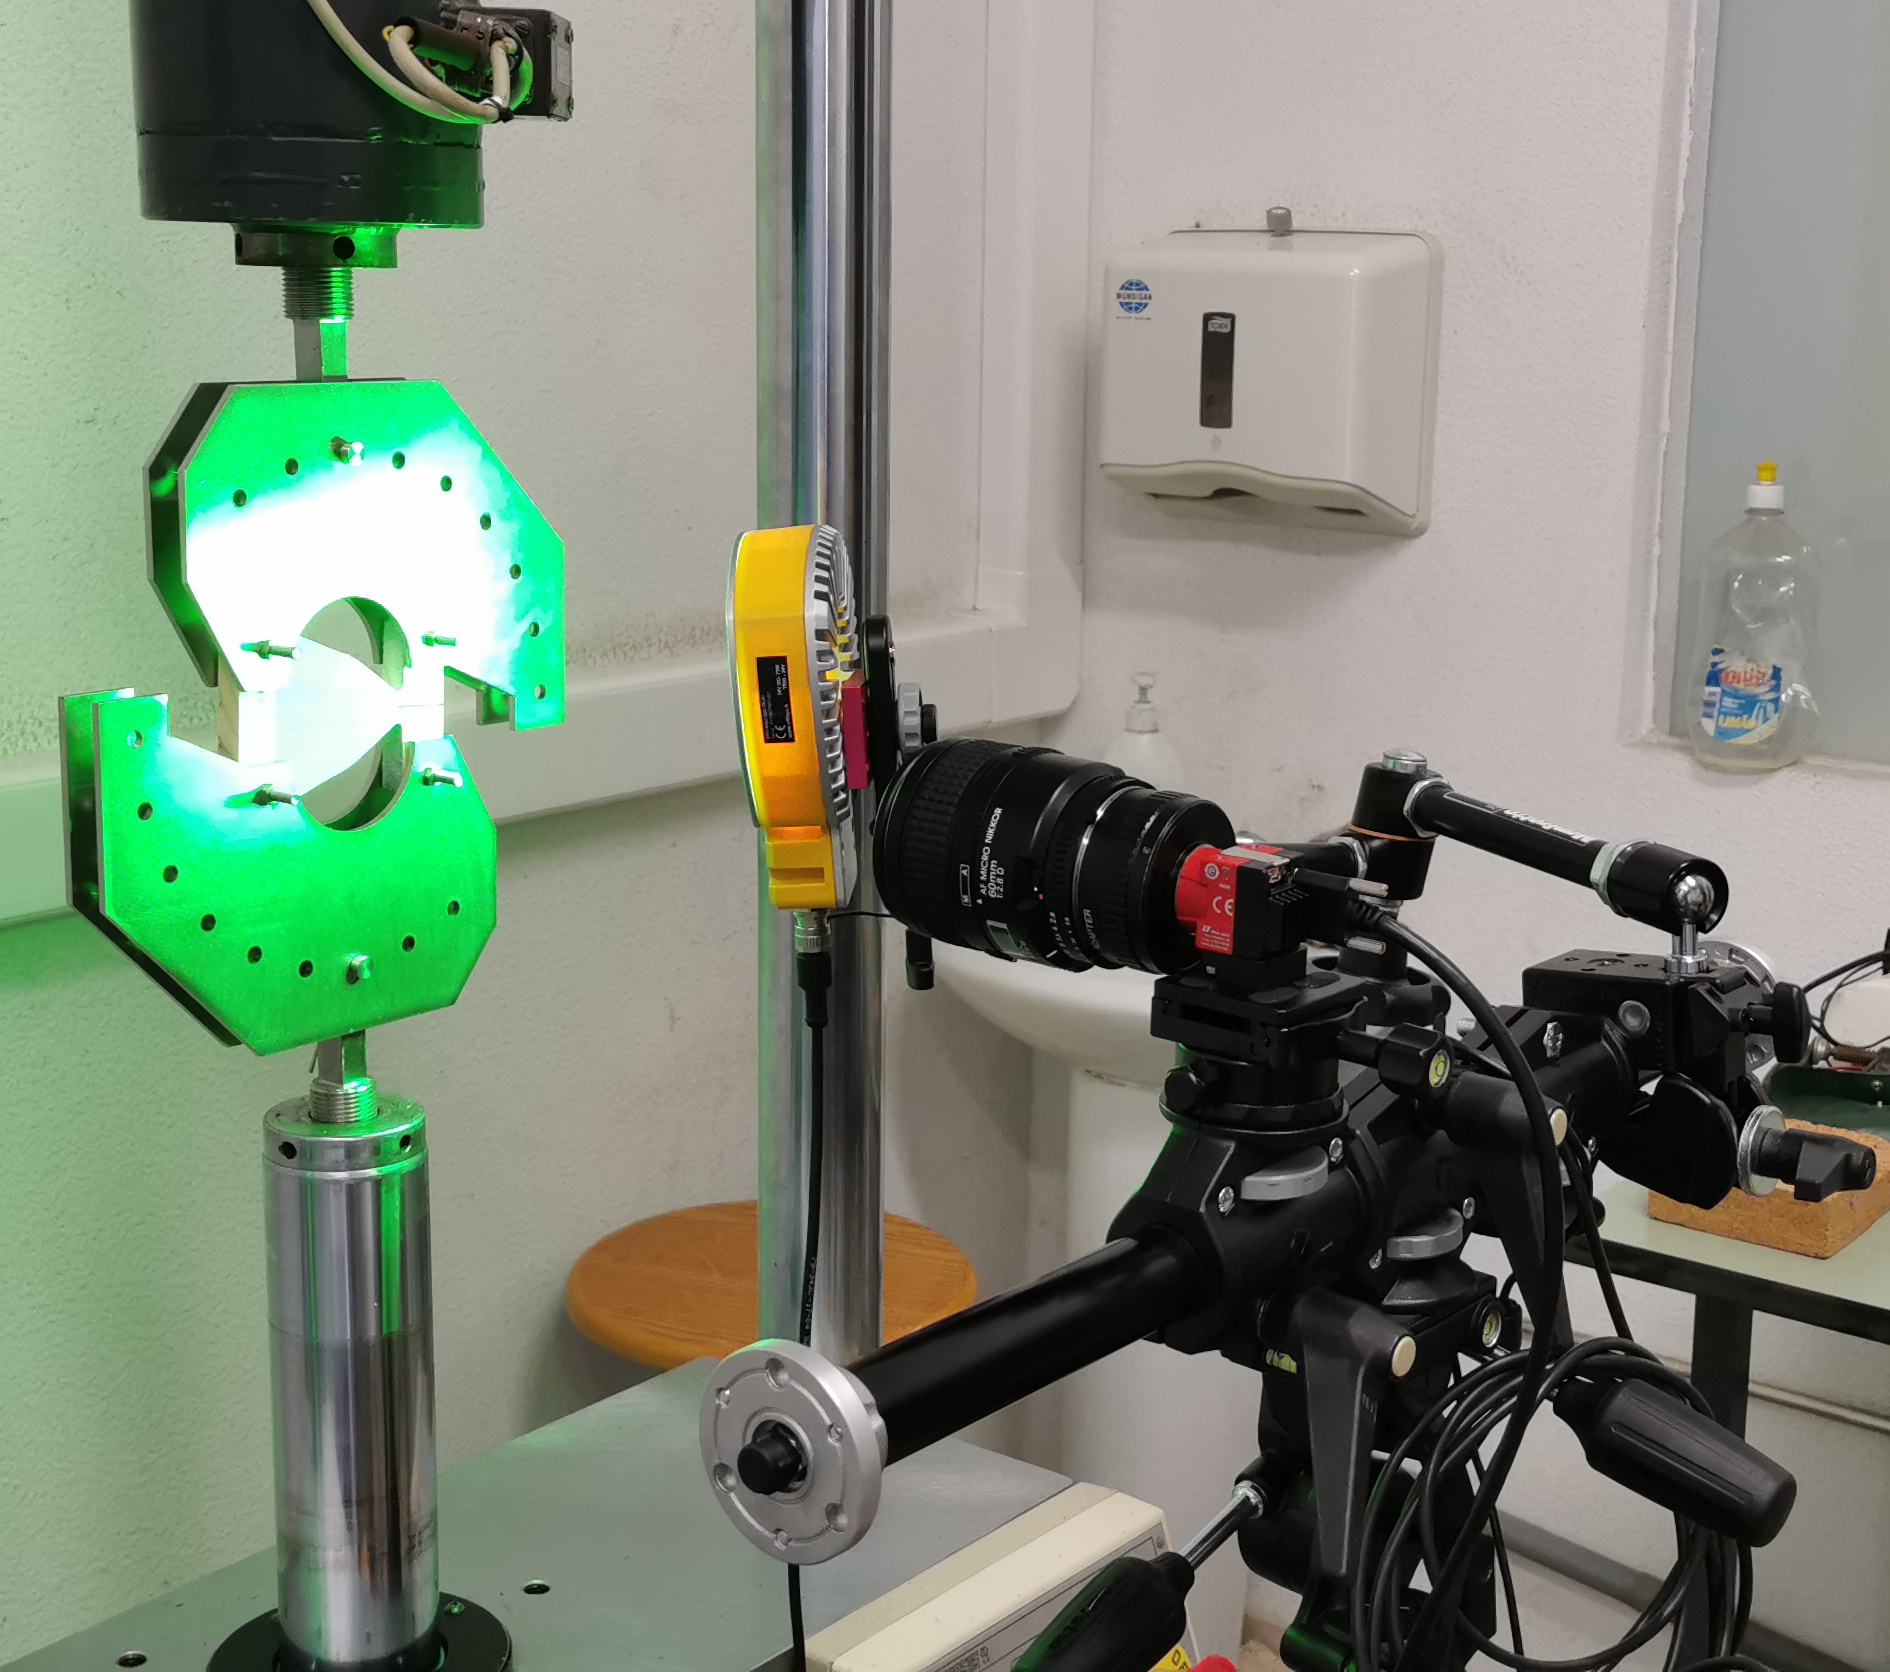
\includegraphics[width=.6\textwidth]{Setup0_crop}
	\caption{Experimental set-up.}
	\label{fig:Setup0°}
\end{figure}


\begin{figure}[htp]
	\centering
	\begin{tabular}{c}
		\includegraphics[width=5cm]{Speckle_DIC} \\
		(a) \\
		\\
		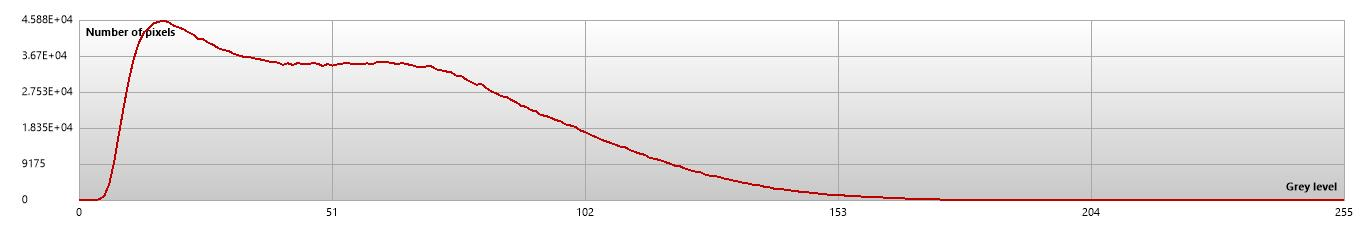
\includegraphics[width=16cm]{histogram} \\
		(b) \\
		\\
	\end{tabular}
	\caption{(a) Speckle pattern typically obtained with DIC; (b) Histogram of the speckle image.}
	\label{fig:Speckle_DIC}
\end{figure}


The selected parameters for the DIC analysis play a crucial role in determining the accuracy and spatial resolution of the measured displacements and reconstructed strain fields \citep{Xavier2012207,PereiraandXavier2018}. Consequently, they are considered fundamental factors. To achieve a trade-off between spatial resolution and accuracy, a parametric analysis was conducted utilizing the Parametric Module of MatchID. The resulting DIC settings are summarized in Table~\ref{tab:MatchID_param}.

The range of values defined in this performance study, including the subset size ($f_s$), subset step, affine and quadratic displacement shape functions, the size of the strain windows, and the order of the polynomial fitting function, is defined by the table \ref{tab:MatchID_param}. It is believed that the pre-selected range of values is reflective of the permissible DIC setup parameter range.

\begin{table}[]
	\centering
	\begin{tabular}{m{.3\textwidth}m{.4\textwidth}}\toprule
		Correlation   Coefficient: & ZNCC \\
		Interpolation order: & Bicubic Splines \\ 
		Transformation order: & Quadratic \\
		Prefiltering: & Gaussian \\
		Progress history: & Spatial \\
		Subset size: & 31 \\
		Step size: & 10 \\
		Strainwindow size: & 5 \\ 
		Virtual Strain Gauge: & 71 pixel \\
		Strain interpolation: & bilinear (Q4) Lagrange polynomials\\
		Strain Convention: & Green-Lagrange \\\bottomrule
	\end{tabular}
	\caption{DIC setting parameters used in the MatchID software for the analyses.}
	\label{tab:MatchID_param}
\end{table}


\section{Results and comparison in mode I}

\subsection{Load-displacement curves}

Normally four distinct parts are observed on a load-displacement curve for Mode I fracture loading:

\begin{itemize}
	\item A small area visible at the beginning of the curve which corresponds to the setting up of the loaded specimen. 
	\item A nearly linear region arises from the elastic loading phase with a static crack front.
	\item The third segment is distinguished by a series of critical force peaks, which signify a distinct crack initiation. The progressive increase in these peaks confirms the crack's stability zone.
	\item Lastly, the final segment entails the material's rupture, which transpires when an ultimate force is applied, marking the instability of the crack.
\end{itemize}

Because of the preload applied at the fixture and specimen adjustments, the raw load and displacements were slightly shifted to reproduce the initial conditions of zero displacements and load at the reference configuration. This extrapolation is possible because the curve has an initial linear regime. All load-displacement curves are summarised in appendix \ref{Appendix1}.


\begin{figure}[htp]
	\begin{minipage}[c]{.46\linewidth}
		\centering
		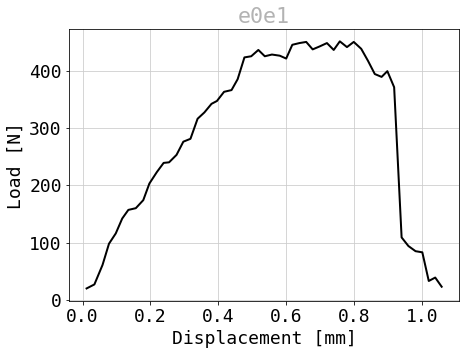
\includegraphics[width=8cm]{P_e0e1}
		\caption{Characteristic load-displacement ($P-\delta$) curve.}
		\label{fig:e0e1_Pdelta}
	\end{minipage}
	\hfill%
	\begin{minipage}[c]{.46\linewidth}
		\centering
		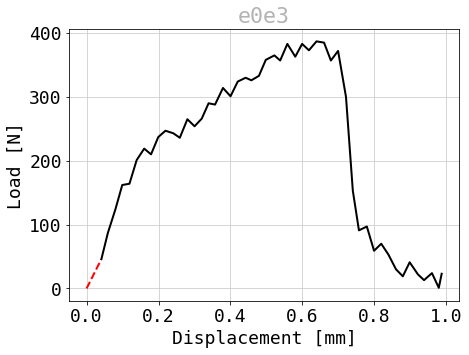
\includegraphics[width=8cm]{P_e0e3}
		\caption{load-displacement ($P-\delta$) curve shifted.}
		\label{fig:e0e5_Pdelta}
	\end{minipage}
\end{figure}


\subsection{Deformation fields}

Typical $y$-component of the strain field ($\epsilon$yy) obtained with the DIC method is shown in Figure \ref{fig:Strain_def}.
During the tests we noticed that the cracks tend to propagate according to the orientation and inclination of the grain, as expected.
In Figure \ref{fig:Strain_def} for specimen e0e1, we assume a small fibre inclination which could explain the observed crack orientation.

\begin{figure}[htp]
	\centering
	\begin{tabular}{c}
		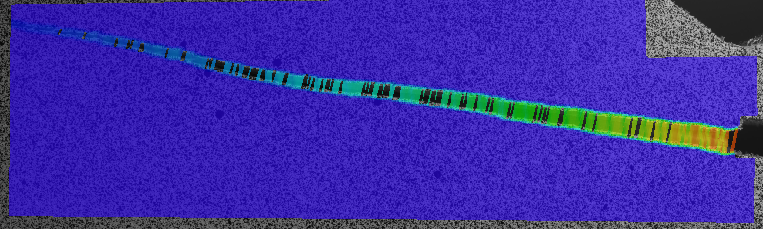
\includegraphics[width=8cm]{e0e1} \\
		e0e1 deformation map \\
		\\
		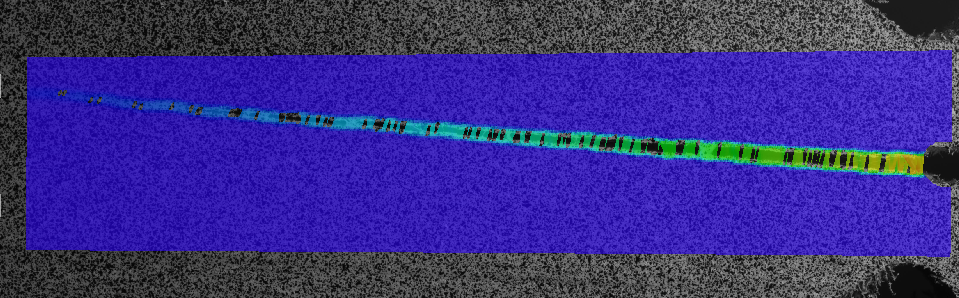
\includegraphics[width=8cm]{e0e2} \\
		e0e2 deformation map \\
		\\
		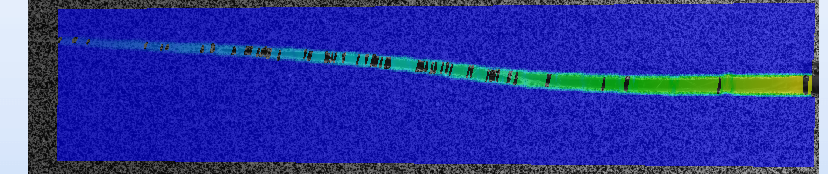
\includegraphics[width=9cm]{e0e3} \\
		e0e3 deformation map \\
	\end{tabular}
	\caption{Typical deformation map ($\epsilon_{yy}$) obtained with DIC.}
	\label{fig:Strain_def}
\end{figure}

Strain maps are employed to track the position of the crack tip at a macroscopic level during the tests. This analysis serves to validate the crack tip position obtained through both the proposed methods 1 and 2. The blue data points in Figures \ref{fig:fig39} and \ref{fig:fig40} correspond to tests e0e2 and e0e3, respectively, and are obtained through graphical interpretation of the $\varepsilon_{yy}$ strain fields. It is evident that the blue points align accurately with the curves generated by method 1, indicating the consistency of this approach. While method 2 appears to have slightly lower accuracy, we will still employ it to determine $G$ and assess the impact of minor variations in $a(t)$.

\begin{figure}[htp]
	\begin{minipage}[c]{.46\linewidth}
		\centering
		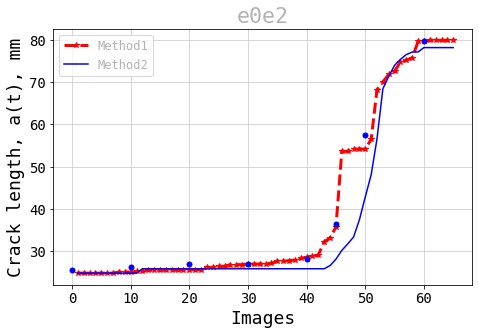
\includegraphics[width=8cm]{e0e2_graphicread}
		\caption{Crack tip by graphic reading e0e2.}
		\label{fig:fig39}
	\end{minipage}
	\hfill%
	\begin{minipage}[c]{.46\linewidth}
		\centering
		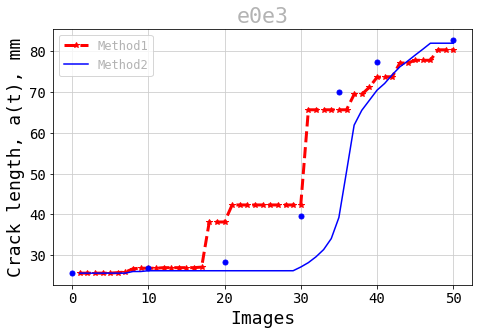
\includegraphics[width=8cm]{e0e3_graphicread}
		\caption{Crack tip by graphic reading e0e3.}
		\label{fig:fig40}
	\end{minipage}
\end{figure}


\subsection{Crack tip opening curves}

The user is required to select a pair of subsets for evaluating CTOD. To ensure precise displacement measurement, the chosen subsets must be positioned as close to the crack tip as possible while avoiding the borders and edges of the new crack surfaces. Based on this study, the databases are updated using the selected COD pair. To visually represent the selected CTOD, a plot was generated, as shown in Figure \ref{fig:CTOD_example}, with the chosen CTOD pair highlighted in blue. Additionally, to demonstrate the utmost precision of the selected COD pair for each specimen, the plot includes a comparison with the curve obtained using the lower and upper COD pairs.

\begin{figure}[htp]
	\centering
	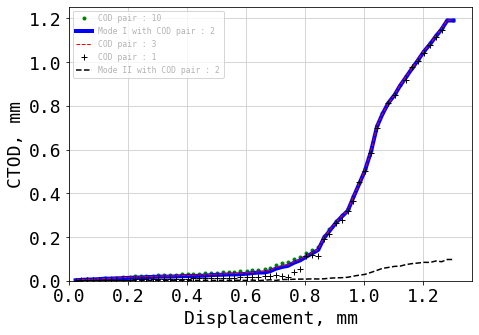
\includegraphics[width=9cm]{CTOD_example}
	\caption{Crack Tip Opening Displacement choice.}
	\label{fig:CTOD_example}
\end{figure}

Figure \ref{fig:COD_modeI} shows the crack opening curves in mode I, representing the displacement of the two surfaces of the crack. These curves exhibit two distinct phases. Initially, there is a phase where the force increases slightly alongside a minor CTOD increment. Subsequently, a second phase follows, characterised by a decrease in load and a rapid CTOD increase. During the first phase, the MMCG specimen effectively withstands the force exerted by the tensile machine, while in the second phase, the crack is already propagating. Consequently, the wood sample offers minimal resistance, leading to a notable force reduction and a significant CTOD increase.
For calculating $G$, only the section of the curve preceding the abrupt decrease in force, denoted as $P$, will be utilised. Taking curve e0e6 as an example, it is observed that the specimen fractures at a CTOD of approximately 1.2 mm, prompted by a sudden decline in force.

\begin{figure}[htp]
	\centering
	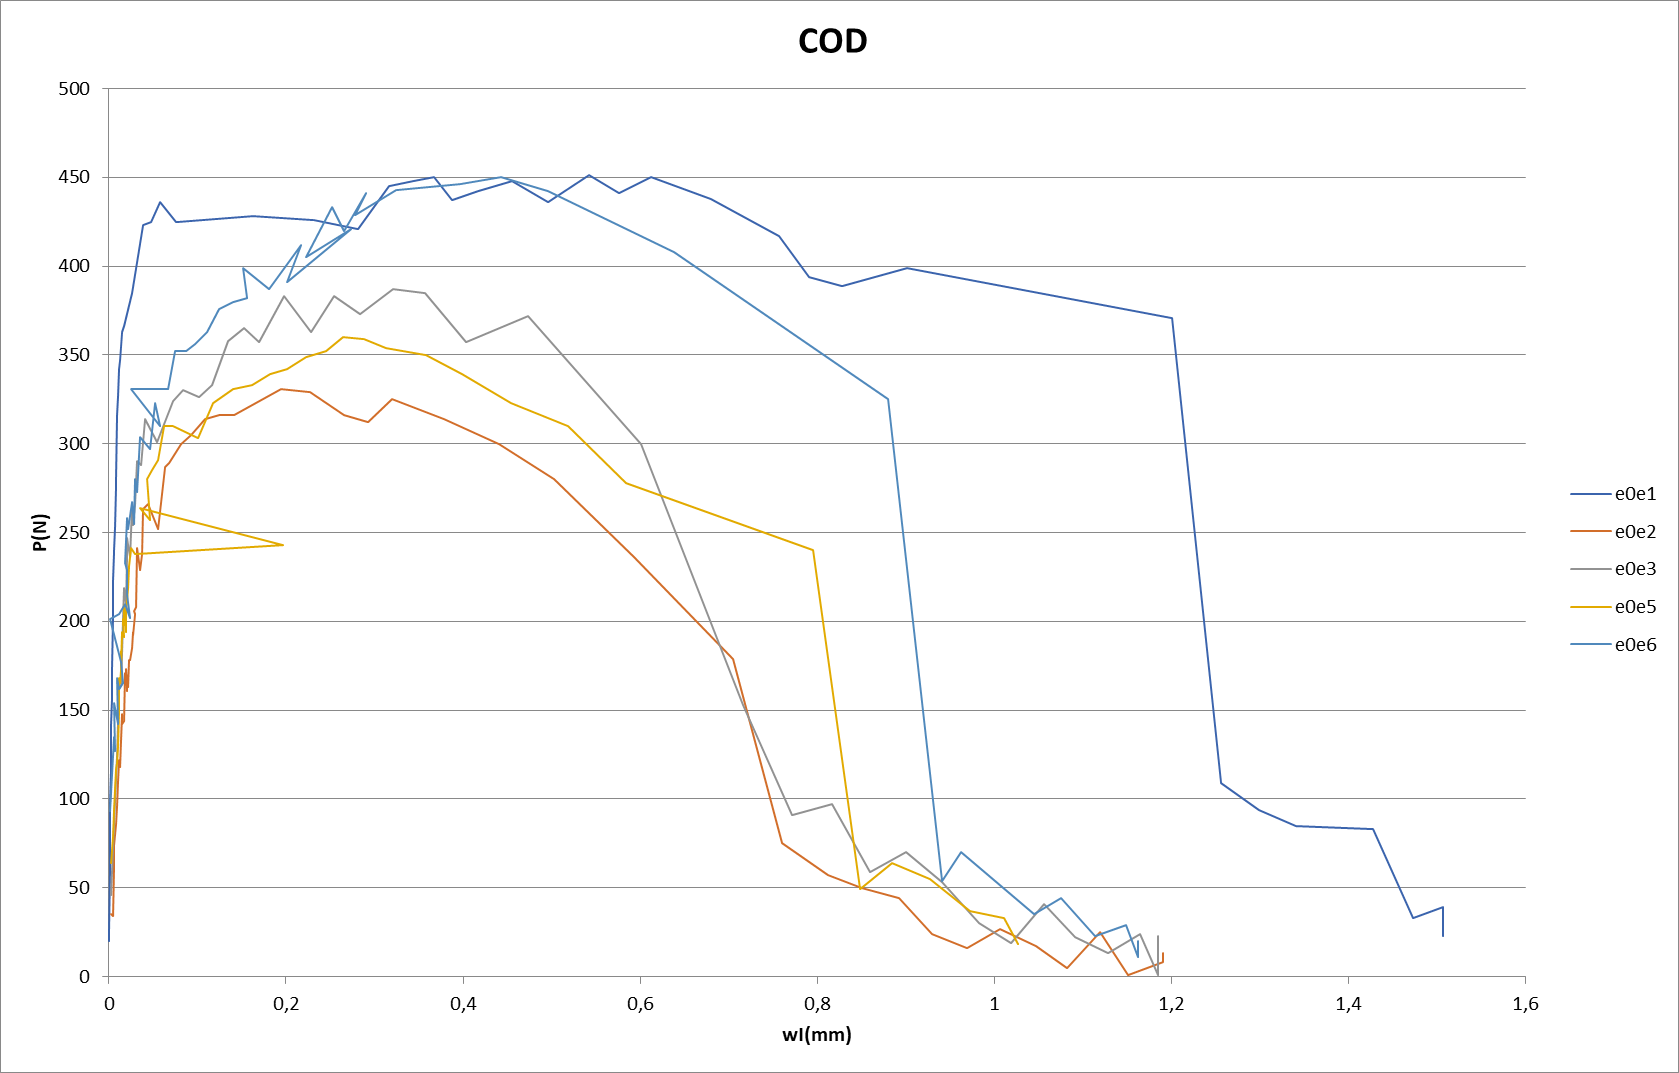
\includegraphics[width=13cm]{COD_modeI}
	\caption{Crack Tip Opening Displacement.}
	\label{fig:COD_modeI}
\end{figure}

\subsection{Crack length curves}

For method 1 by compiling the evolution of $a(t)$ as a function of the images recorded for several $\alpha$ values (\ref{fig:Cracklength_modeI_example}), it is possible to get an idea of the $\alpha$ value required to obtain the best $a(t)$. Indeed, the $\alpha$ parameter must be as small as possible for the evolution of the crack length to be complete. So, for each crack length in the sample, it is possible to eliminate several candidates. In this example \ref{fig:Cracklength_modeI_example}, it is possible to eliminate the use of curves with $a(t)<70$ mm. These $\alpha$ values do not allow the entire crack length to be studied. To distinguish between the black and turquoise curves, you can place the position of the crack tip with a red dot on the displacement map. Then for different stages, we can then see which curve corresponds best to the position of the crack tip. Here, the black curve was chosen.

To obtain $a(t)$ using method 2, we need to read $a_1$ and $a_f$ graphically and choose a pair of COD lines that are not damaged by nans values.

\begin{figure}[H]
	\centering
	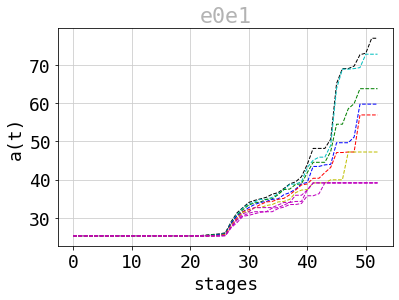
\includegraphics[width=9cm]{Cracklength_modeI_example}
	\caption{Crack length evolution depending on alpha.}
	\label{fig:Cracklength_modeI_example}
\end{figure}

Figure \ref{fig:crack_method1} and \ref{fig:crack_method2} present all the crack length curves corresponding to mode I displacement. In method 1, the expected presence of distinct plateaus in the crack length is observed. The crack length progressively and continuously increases before reaching rupture. The design of the MMCG specimen facilitates stable crack propagation, where cracks propagate slowly until failure occurs at maximum load. Some images show bridges defining a damaged fracture process zone. Extending the crack from these fibre bridging allows for continuous crack propagation. Analysing all the crack length propagation plots is interesting. The curves exhibit similar shapes, and the crack ends at approximately the same length. The variation lies in the stage at which crack propagation initiates. For example, in method 1, e0e1 begins crack propagation at stage 23, whereas e0e2 starts at stage 9.

In contrast, method 2 yields similar curves to method 1, but they appear smoother. However, this smoothness is not necessarily advantageous as crack propagation in wood typically occurs in a more step-by-step manner. Furthermore, upon checking Figure \ref{fig:a_e0e1} or Figure \ref{fig:a_e0e2} in the appendix, it can be observed that the crack length in method 2 is generally smaller than that in method 1 for the same stage.

\begin{figure}[htp]
	\centering
	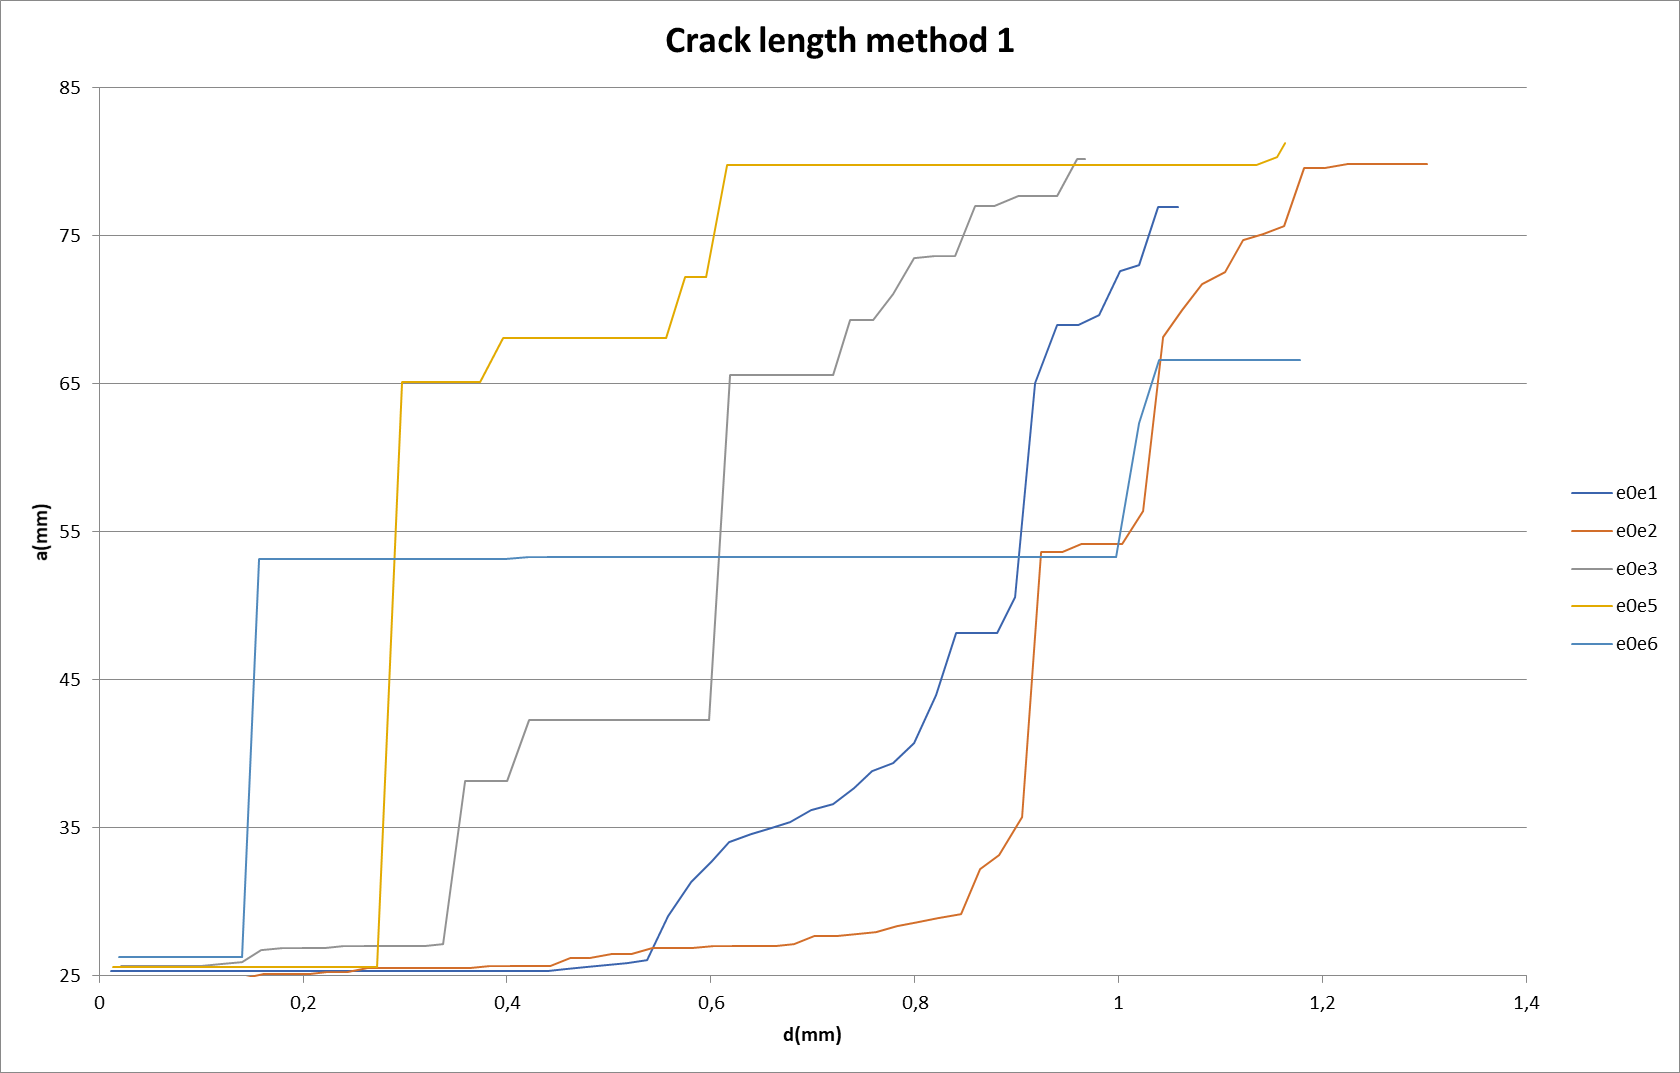
\includegraphics[width=13cm]{crack_method1}
	\caption{Crack length evolution method 1.}
	\label{fig:crack_method1}
\end{figure}

\begin{figure}[htp]
	\centering
	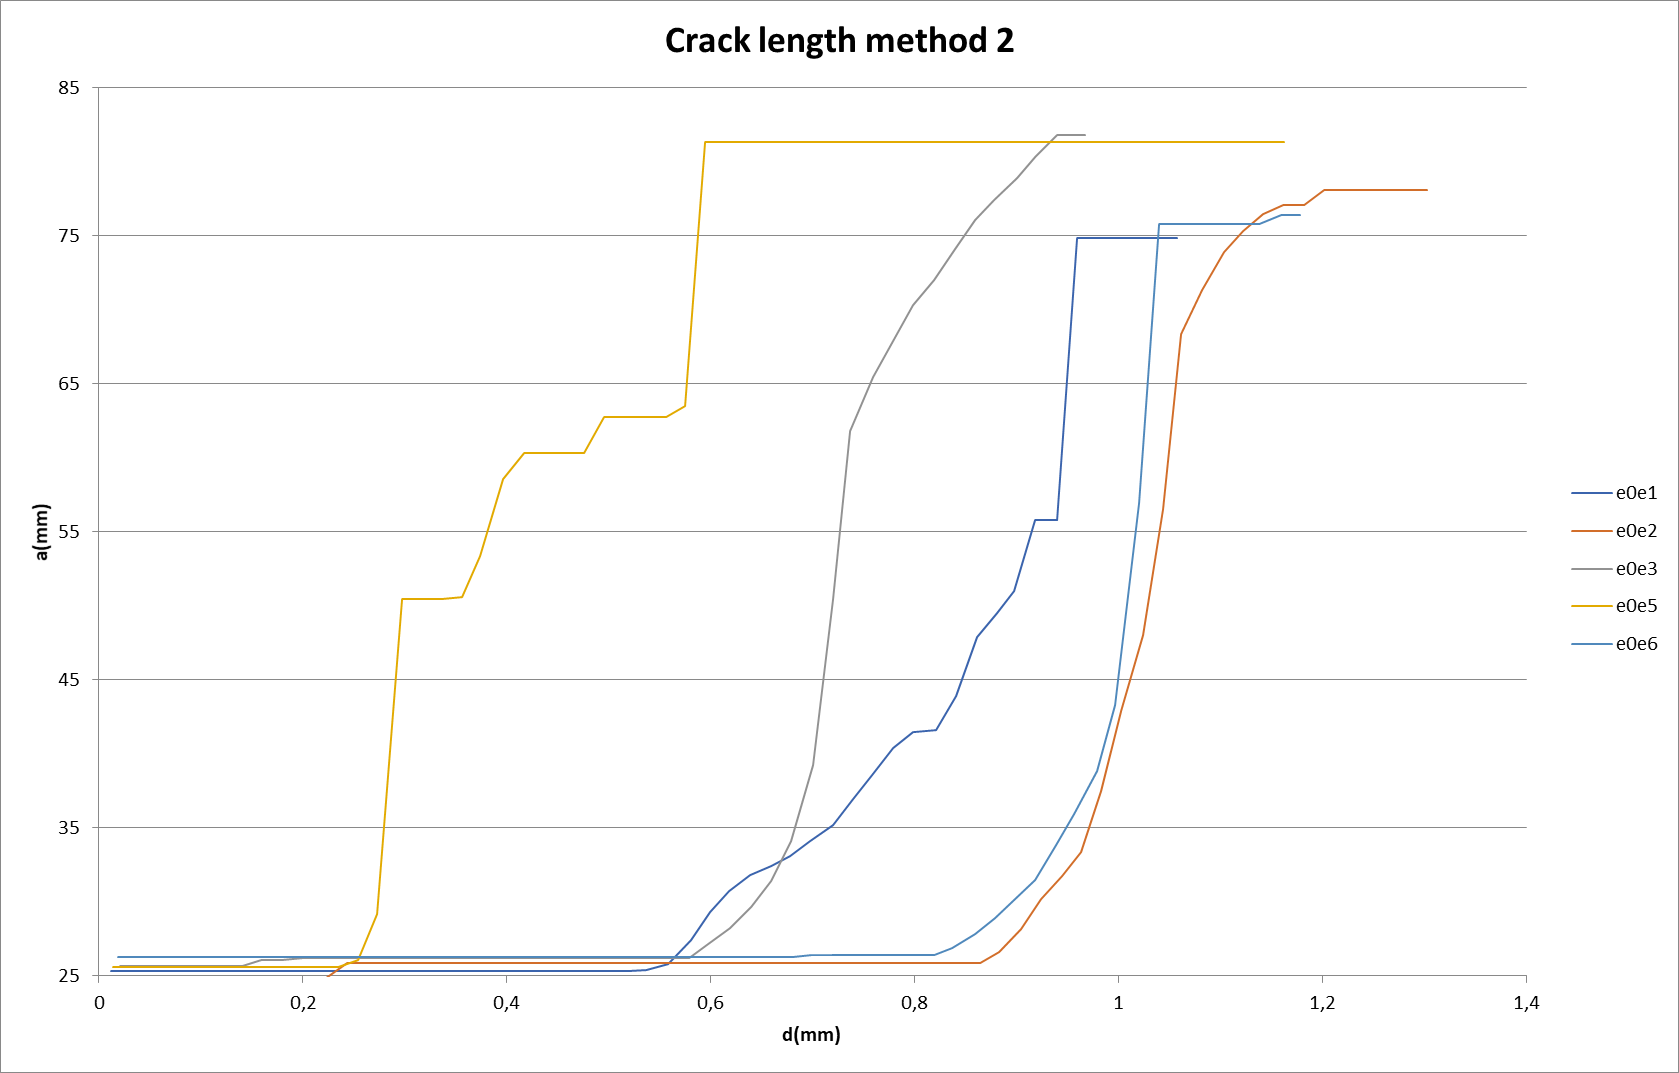
\includegraphics[width=13cm]{crack_method2}
	\caption{Crack length evolution method 2.}
	\label{fig:crack_method2}
\end{figure}

\subsection{Critical energy release rate}

Several methods can be employed to calculate the energy release rate, as described in Equation \ref{eq:eq125}. Compliance can be determined in various ways. One approach, used by Malfait et al. (2021) and Moutou-Pitti (2008), involves calculating the $\Delta c$ between the starting point and the considered point for all critical forces. These critical forces correspond to points where the force decreases in subsequent stages, indicating crack propagation, according to Moutou-Pitti (2008). Another possibility is to determine $C$ as an interpolated function, such as $C(a)=m*a(t)^3+n$, where $a(t)$ represents the crack length. The derivative of compliance with respect to crack length can then be used. Both methods were tested to determine the most suitable approach, and ultimately, $\Delta c$ was used to calculate $G$. However, the cubic function employed did not accurately pass through all the points on the $C$ versus $a(t)$ graph, resulting in significant inaccuracies. The calculated values of $G$ using this method were on the order of $10^3 J/m^2$, which is excessively high.

Figures \ref{fig:G_method1} and \ref{fig:G_method2} present the values of $G$ obtained using the two methods for calculating crack length. Notably, different specimens reach varying values of $a(t)$ at the maximum energy release rate ($G_\text{Imax}$). Method 1 and Method 2 achieve $G_\text{Imax}$ for $a(t)$ within the range of 33 to 80 mm, with a tendency for Method 1 to correspond to $a(t)$ of approximately 60 mm. Method 2 yields $G_\text{Imax}$ at shorter crack lengths. This discrepancy can be attributed to the generally smaller values of $a(t)$ for the same stage in Method 2.


\begin{figure}[htp]
	\centering
	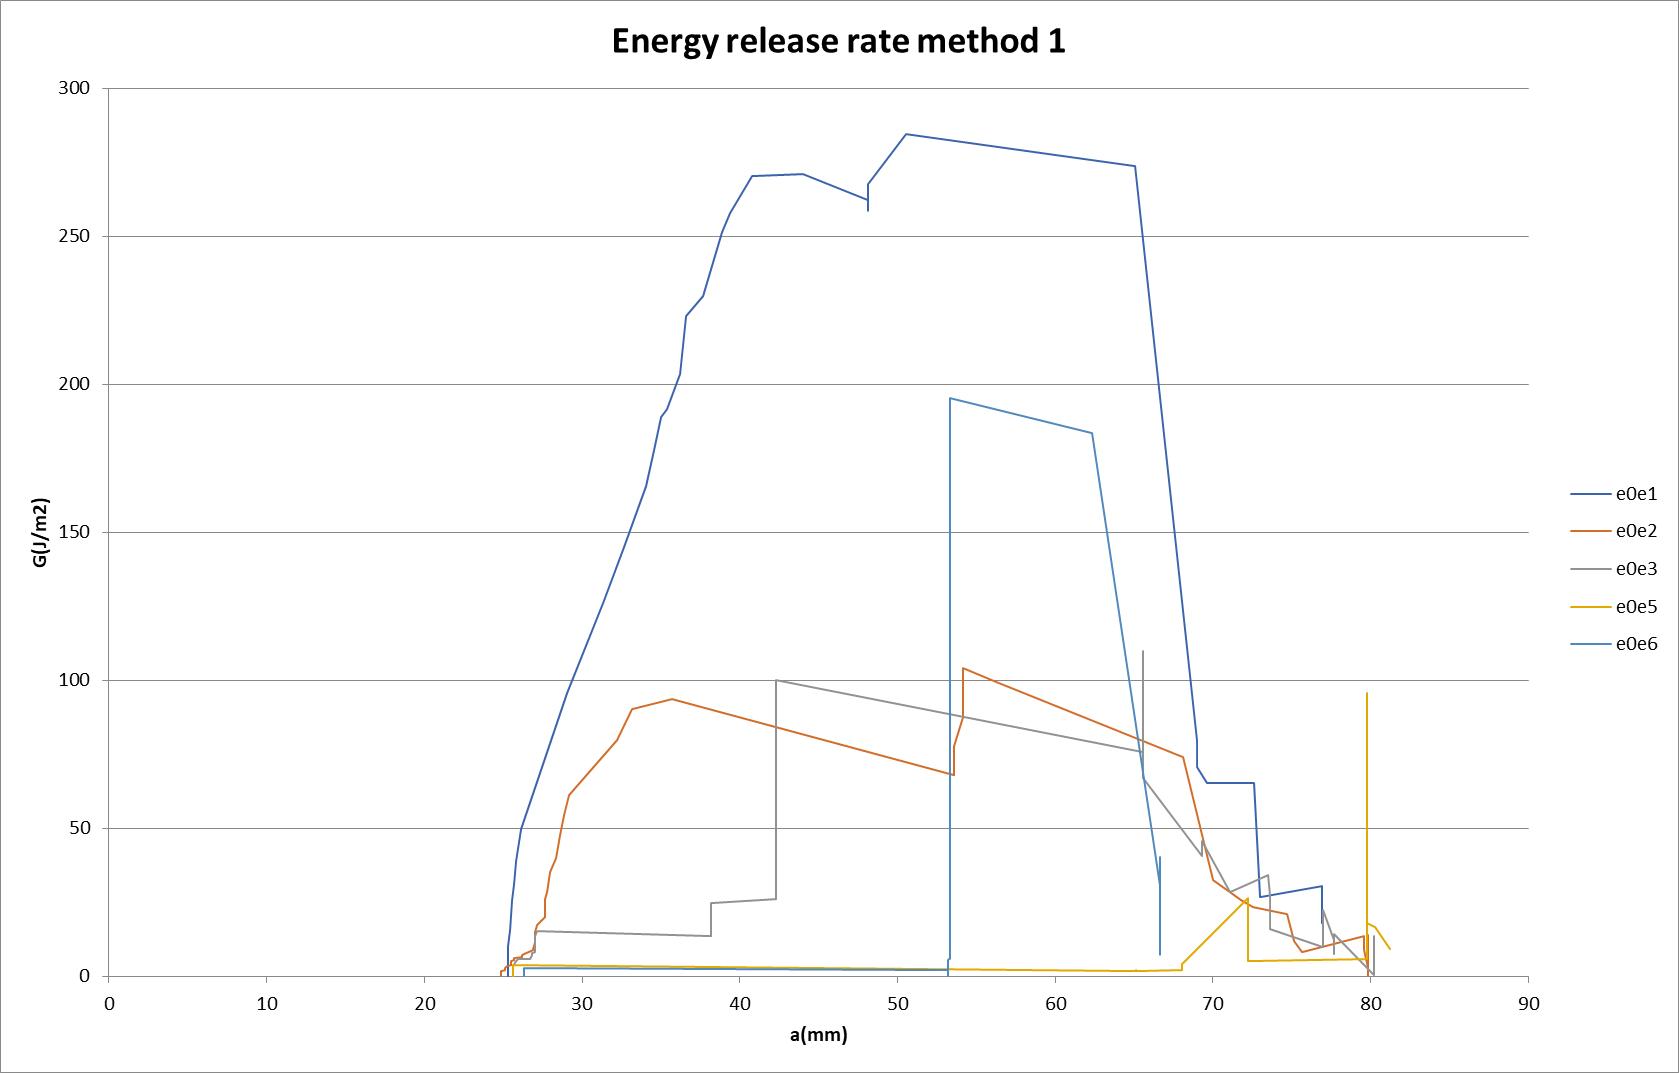
\includegraphics[width=13cm]{G_method1}
	\caption{$G$ obtaiend from method 1.}
	\label{fig:G_method1}
\end{figure}

\begin{figure}[htp]
	\centering
	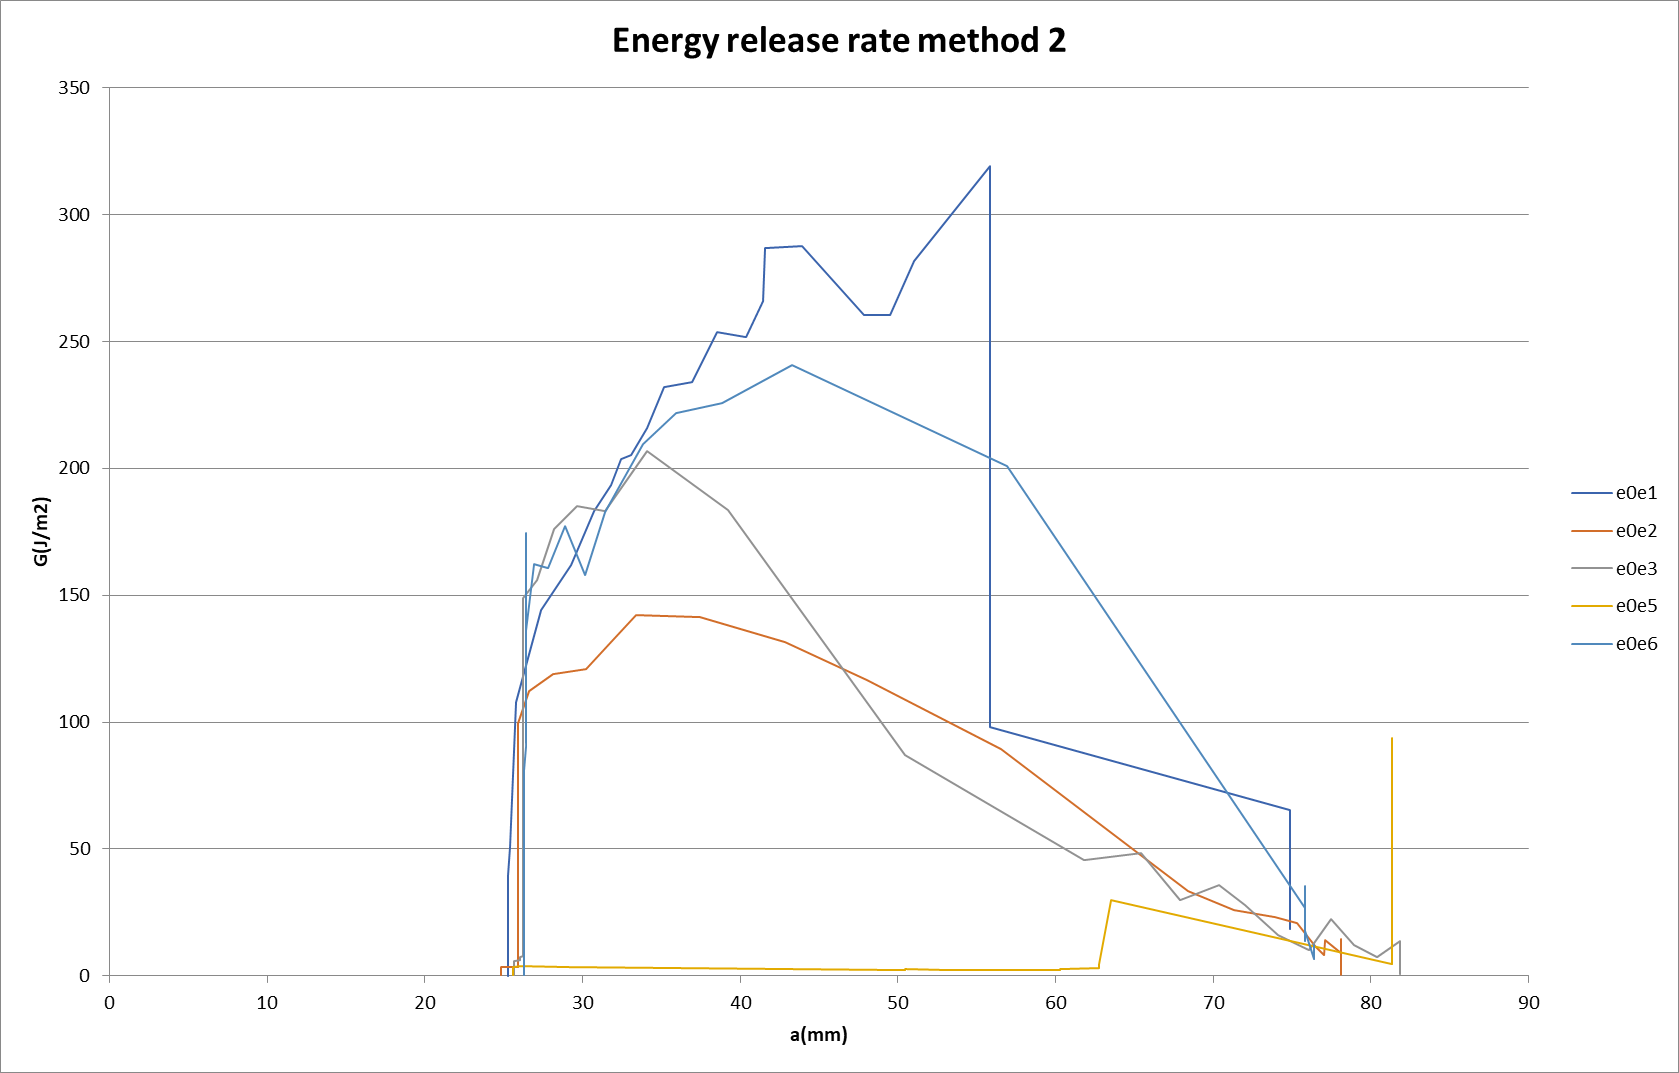
\includegraphics[width=13cm]{G_method2}
	\caption{$G$ obtaiend from method 2.}
	\label{fig:G_method2}
\end{figure}

It is evident that $G$ exhibits a gradual increase with Method 1, and Figure \ref{fig:G_method1} bears resemblance to the $G$ plots obtained by Odounga (2018) in their doctoral dissertation. In contrast, with Method 2, it appears that $G$ experiences more rapid growth for a smaller increment in $a(t)$. Notably, for a given testing period, Method 1 generally yields higher $a(t)$ values compared to Method 2. This finding demonstrates that even a slight variation in crack length measurement can yield vastly different $G$ results. Additionally, the observed trend of the plots reaching a plateau aligns with the expected curve shape.
The individual figures of $G$ can be found in Appendix \ref{Appendix1}, facilitating a comprehensive examination of the curve shape for each specimen.
Table \ref{fig:tableG1} presents the maximum values of $G$ in mode I for silver Fir. It is evident that Method 2 tends to yield higher $G$ values, which can be attributed to a lower estimate of $a(t)$ for the same image or stage.

\begin{table} [H]
	\centering
	\begin{tabular}{ccccccc}
		\toprule % horizontal line at the top of the table
		&  & e0e1 & e0e2 & e0e3 & e0e5 & e0e6\\\midrule
		& Method 1: $G_\text{Imax}$ ($J/m^2$) & 284.44 & 90.24 & 107.49 & 95.67 & 183.58 \\
		& Method 2: $G_\text{Imax}$ ($J/m^2$) & 286.65 & 131.16 & 206.73 & 93.83 & 199.59 \\\bottomrule
	\end{tabular}
	\caption{$G_\text{Imax}$ values for Silver Fir specimens in mode I.}
	\label{fig:tableG1}
\end{table}

\subsection{Discussion}

Table \ref{fig:fig37} compares the maximum energy release rate values obtained in this study with those reported in the literature. The comparison focuses on temperate species with similar density, moisture content ranging between 9% and 12%, and an initial crack oriented in the radial-longitudinal (RL) direction. Silver fir's average maximum energy release rate is highlighted in bold and compared to different species and test methods, including 2MCG, DCB, and Wedge Splitting tests.
Firstly, it is noteworthy that the magnitude of $G$ for silver fir is within the same order of magnitude as other species. Silver fir exhibits a difference of 29% compared to alder, 36% compared to Pinus pinaster, and 33% compared to Padouk. Moreover, similar values have been reported in the work of Odounga (2018), albeit with a standard deviation 2 to 3 times greater, indicating more dispersed results.
In the study by Xavier et al. (2014), experimental values of $G=190$ J/m² were also obtained, which aligns with the results of this study. Additionally, alder and Pinus pinaster exhibit similar densities (around 0.1) in comparison to silver fir.
The observed scattering of results can be attributed to the inherent material properties of wood, which is known for its high natural variability and anatomical composition. Furthermore, different energy release rate measurement methods and experimental parameter variations inevitably impact the final results.
It is worth mentioning that the specimens in this study were predominantly derived from the extremity of the tree trunk rather than the central portion. The inclination of tree rings is apparent when observing our specimens, which could explain the slightly lower value obtained in our tests since $G_{RL} > G_{TL}$, as demonstrated in the article by Reiterer (2002).

\begin{table}[H]
	\centering
	\resizebox{\textwidth}{!}{
		\begin{tabular}{cccccccc}
			\toprule % ligne horizontale en haut du tableau
			& References & Wood species & Test type & Orientation & Density & $G_{\max}(J/m^2)$ & Standard deviation \\
			\midrule
			& & \textbf{Silver fir} & \textbf{2MCG} & \textbf{RL} & \textbf{0.43} & \textbf{170} & \textbf{77} \\
			\midrule
			& \cite{Angellier2017} & Douglas fir & DCB & RL & 0.54 & 784 &  \\
			\midrule
			& \cite{Angellier2017} & White fir & DCB & RL & 0.49 & 570 &  \\
			\midrule
			& \cite{Xavieretal2014} & Pinus Pinaster & DCB & RL & 0.543 & 270 & 64 \\
			\midrule
			& \cite{Reiterer2002} & Spruce & WS & RL & 0.479 & 337 & 47 \\
			\midrule
			& \cite{Reiterer2002} & Alder & WS & RL & 0.510 & 244 & 41 \\
			\midrule
			& \cite{Reiterer2002} & Oak & WS & RL & 0.553 & 348 & 38 \\
			\midrule
			& \cite{Reiterer2002} & Ash & WS & RL & 0.701 & 551 & 38 \\
			\midrule
			& \cite{Odounga2018phd} & Okoumé & 2MCG & RL & 0.39-0.5 & 317 & 160 \\
			\midrule
			& \cite{Odounga2018phd} & Iroko & 2MCG & RL & 0.56-0.7 & 323 & 200 \\
			\midrule
			& \cite{Odounga2018phd} & Padouk & 2MCG & RL & 0.7-0.88 & 255 & 200 \\
			\bottomrule % ligne horizontale en bas du tableau
		\end{tabular}
	}
	\caption{Comparison of mean max G values for specimens in the literature, 2MCG: Mixed Mode Crack Growth, DCB: Double Cantilever Beam, WS: Wedge Splitting test, RL: Radial Longitudinal.}
	\label{fig:fig37}
\end{table}


\section{Conclusion}

In this study, cracking tests were carried out on a softwood, Silver Fir. A speckle pattern was transferred to each specimen to follow the progress of the crack front and measure its opening. Two methods were used and compared to measure the crack front. It seems that method 1 is more effective than method 2. The variables obtained from the DIC method were used to calculate the critical energy release rate for each specimen using the compliance method. Comparison of the $G_\text{Imax}$ averages with those for temperate species given in the literature review shows that the results obtained are similar, although slightly lower.